\documentclass[uplatex,dvipdfmx,a4paper,10pt]{jsarticle}
\usepackage{graphicx}
\usepackage{amsmath}
\usepackage{latexsym}
\usepackage{multirow}
\usepackage{url}
\usepackage[separate-uncertainty]{siunitx}
\usepackage{physics}
\usepackage{enumerate}
\usepackage{bm}
\usepackage{pdfpages}
\usepackage{pxchfon}
\usepackage{tikz}
\usepackage{float}
\usepackage{listings}

% lstlistingのsetting
\lstset{
    basicstyle={\ttfamily},
    identifierstyle={\small},
    commentstyle={\smallitshape},
    keywordstyle={\small\bfseries},
    ndkeywordstyle={\small},
    stringstyle={\small\ttfamily},
    frame={tb},
    breaklines=true,
    columns=[l]{fullflexible},
    numbers=left,
    xrightmargin=0zw,
    xleftmargin=3zw,
    numberstyle={\scriptsize},
    stepnumber=1,
    numbersep=1zw,
    lineskip=-0.5ex
}

% tikz setting
\usepackage{tikz}
\usetikzlibrary{automata, intersections, calc, arrows, positioning, arrows.meta}

% theories setting (for japanese language)
\usepackage{amsmath}
\usepackage{amsthm}

\theoremstyle{definition}
\newtheorem{thm}{定理}[section]
\newtheorem{lem}[thm]{補題}
\newtheorem{prop}[thm]{命題}
\newtheorem{cor}[thm]{系}
\newtheorem{ass}[thm]{仮定}
\newtheorem{conj}[thm]{予想}
\newtheorem{dfn}[thm]{定義}
\newtheorem{rem}[thm]{注}

\newtheorem*{thm*}{定理}
\newtheorem*{lem*}{補題}
\newtheorem*{prop*}{命題}
\newtheorem*{cor*}{系}
\newtheorem*{ass*}{仮定}
\newtheorem*{conj*}{予想}
\newtheorem*{dfn*}{定義}
\newtheorem*{rem*}{注}

% \renewcommand{\rmdefault}{pplj}
% \renewcommand{\sfdefault}{phv}

\setlength{\textwidth}{165mm} %165mm-marginparwidth
\setlength{\marginparwidth}{40mm}
\setlength{\textheight}{225mm}
\setlength{\topmargin}{-5mm}
\setlength{\oddsidemargin}{-3.5mm}
% \setlength{\parindent}{0pt}

\def\vector#1{\mbox{\boldmath $#1$}}
\newcommand{\AmSLaTeX}{%
 $\mathcal A$\lower.4ex\hbox{$\!\mathcal M\!$}$\mathcal S$-\LaTeX}
\newcommand{\PS}{{\scshape Post\-Script}}
\def\BibTeX{{\rmfamily B\kern-.05em{\scshape i\kern-.025em b}\kern-.08em
 T\kern-.1667em\lower.7ex\hbox{E}\kern-.125em X}}
\newcommand{\DeLta}{{\mit\Delta}}
\renewcommand{\d}{{\rm d}}
\def\wcaption#1{\caption[]{\parbox[t]{100mm}{#1}}}
\def\rm#1{\mathrm{#1}}
\def\tempC{^\circ \rm{C}}

\makeatletter
\def\section{\@startsection {section}{1}{\z@}{-3.5ex plus -1ex minus -.2ex}{2.3ex plus .2ex}{\Large\bf}}
\def\subsection{\@startsection {subsection}{2}{\z@}{-3.25ex plus -1ex minus -.2ex}{1.5ex plus .2ex}{\normalsize\bf}}
\def\subsubsection{\@startsection {subsubsection}{3}{\z@}{-3.25ex plus -1ex minus -.2ex}{1.5ex plus .2ex}{\small\bf}}
\makeatother

\makeatletter
\def\@seccntformat#1{\@ifundefined{#1@cntformat}%
   {\csname the#1\endcsname\quad}%      default
   {\csname #1@cntformat\endcsname}%    enable individual control
}

% proof enviroment
\renewenvironment{proof}[1][\proofname]{\par
  \pushQED{\qed}%
  \normalfont \topsep6\p@\@plus6\p@\relax
  \trivlist
  \item\relax
  {\bfseries
  #1\@addpunct{.}}\hspace\labelsep\ignorespaces
}{%
  \popQED\endtrivlist\@endpefalse
}
\makeatother

\newcommand{\tenexp}[2]{#1\times10^{#2}}


\begin{document}
% タイトル
\begin{center}
{\Large{\bf 情報工学工房第5回レポート}} \\
{\bf 電気通信大学 Ⅰ類 コンピュータサイエンスプログラム 3年} \\
{\bf 2311081 木村慎之介} \\
\end{center}

\section{無限小の考察}
\hspace{1em}このレポートでは無限小について、アップと1のゲーム木を描画して、直感的に考えられることについて記す。

\subsection{整数}
\hspace{1em}整数とみなせる局面を以下のように定義する。

\begin{dfn}
    局面の値整数\(n\)を以下のように定義する。

    \begin{equation}
        n \simeq \{n-1 | \}
    \end{equation}

    ただし、\(0 = \{ | \}\)と基底を定義する。
    \label{dfn_int}
\end{dfn}

この定義から整数の局面は\(o(n) = \mathcal{L}\)となることがわかる。
ただし、\(n = 0\)のときは\(o(0) = \mathcal{P}\)となる。

\subsection{スター}
\hspace{1em}スターは以下のように定義される。

\begin{dfn}
    局面の値スター\(*n\)を以下のように定義する。

    \begin{equation}
        *n = \{*0, *1, \cdots, *(n-1) |*0, *1, \cdots, *(n-1) \}
    \end{equation}

    ただし、\(*0 = \{ | \}\)と定義する。
    \label{dfn_star}
\end{dfn}

このスターは\(n = 0\)の時に\(\mathcal{P}\)局面、\(n \neq 0\)の時に\(\mathcal{N}\)局面であるから、不偏ゲームのニムをゲーム木で表したものであると認識できる。

\subsection{アップ}
\hspace{1em}アップは以下のように定義される。

\begin{dfn}
    局面の値アップ\(\uparrow\)を次のように定義する。
    
    \begin{equation}
        \uparrow \simeq \{0 | *\}
    \end{equation}
    \label{dfn_up}
\end{dfn}

\noindent アップについて木構造で表すと以下の図のようになる。

\begin{figure}[H]
    \centering
    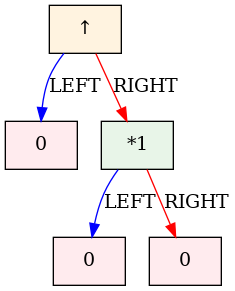
\includegraphics{figure/up.png}
    \caption[width=\textwidth]{アップのゲーム木の木構造}
    \label{figure_up_tree}
\end{figure}

図からもわかるとおり、\(o(\uparrow) = \mathcal{L}\)であることがわかる。

\subsection{アップと1の関係}
\hspace{1em}アップは\(1\)に対して無限小となることが知られている。
この関係を実際にゲームの木構造を見ながら考察していく。

まず\(1\)の局面を木で表現した図を載せる。

\begin{figure}[H]
    \centering
    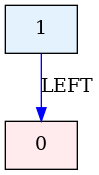
\includegraphics{figure/1.png}
    \caption{\(1\)のゲーム木}
    \label{figure_one_tree}
\end{figure}

次にアップの整数倍の木構造を4つ載せる。
なお、この木構造は標準化されて木構造であることに注意する。

\begin{figure}[H]
    \centering
    \begin{tabular}{cc}
        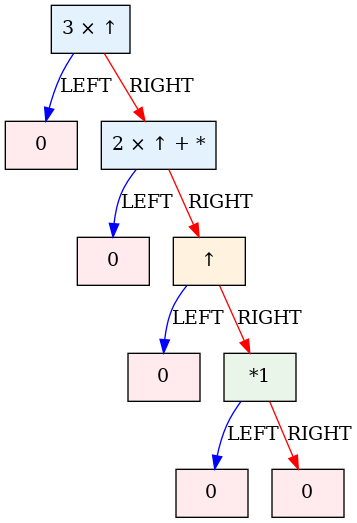
\includegraphics[width=0.3\textwidth]{figure/up_3.png} &
        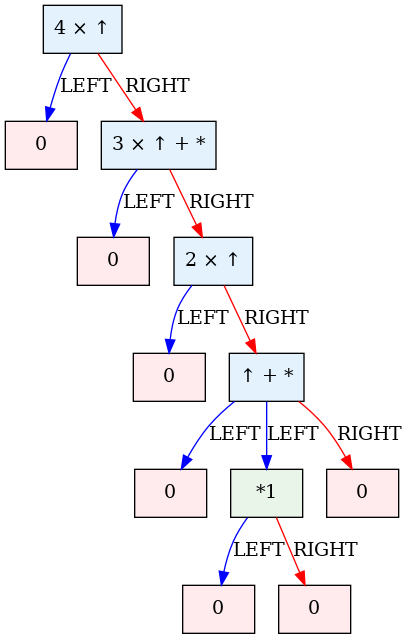
\includegraphics[width=0.3\textwidth]{figure/up_4.png} \\
        \makebox[0.3\textwidth]{(a) 3×↑のゲーム木} &
        \makebox[0.3\textwidth]{(b) 4×↑のゲーム木} \\[1em]
        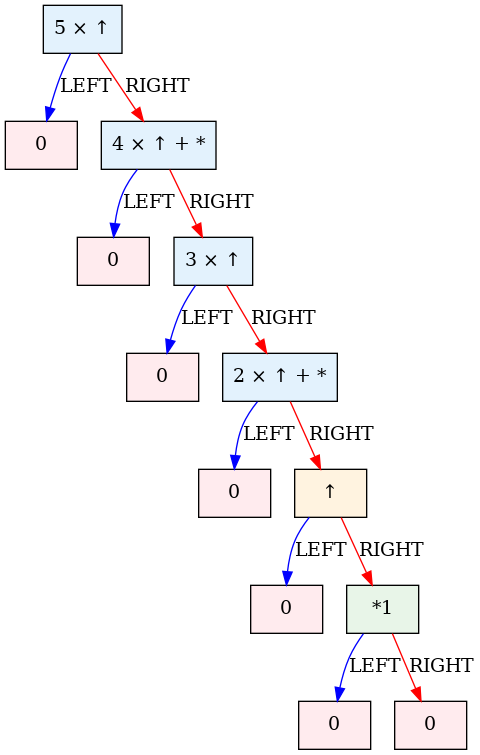
\includegraphics[width=0.3\textwidth]{figure/up_5.png} &
        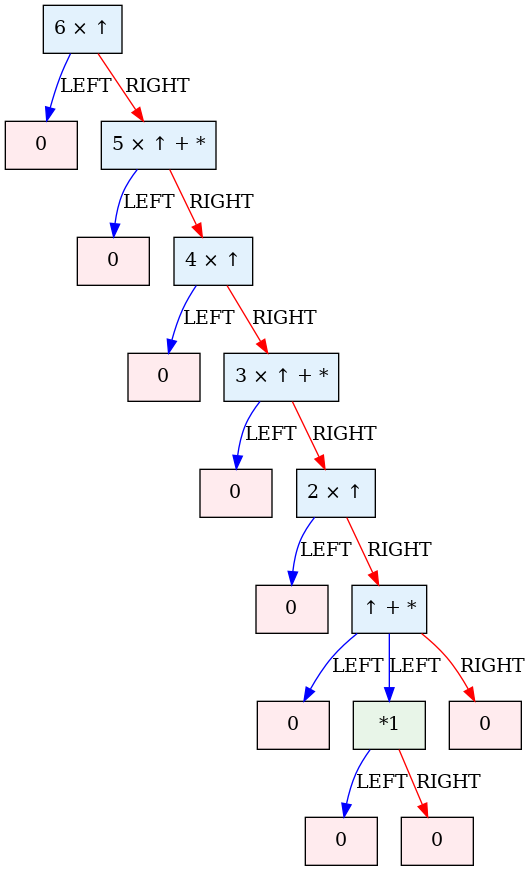
\includegraphics[width=0.3\textwidth]{figure/up_6.png} \\
        \makebox[0.3\textwidth]{(c) 5×↑のゲーム木} &
        \makebox[0.3\textwidth]{(d) 6×↑のゲーム木}
    \end{tabular}
    \caption{アップの整数倍のゲーム木構造}
    \label{figure_up_multiples}
\end{figure}

図より、\(n\)倍のアップの局面は左が勝つものの、誕生日が\(1\)の局面より冗長になっている、つまり左が勝つまでに時間がかかるということがわかる。
このことより、局面の値\(a\)が局面の値\(b\)にたいして無限小であるとは\(a\)の\(n\)倍の局面が勝つためには\(b\)よりもより長い時間をかける必要があると捉えられる。

\subsection{\(n\)を無限にした時の挙動}
\hspace{1em}非不偏ゲームでは有限のものを対象とするため以降の議論は的を外れるかもしれないが、以上の無限小の内容から考えたことを述べる。

仮に\(n\)を無限大に飛ばすことが可能であることを可能としたとき、\(\infty \times \uparrow\)は左右両者が最善の手を打つとゲームの勝ち負けが決まらなくなることが考えられる。
しかしながら少なくとも有限の場合に置いて左に必勝戦略があることから、左が勝ちやすいと考えることができる。
このように無限の場合に置いても、勝敗を完全に決定することができないにせよ、どちらが勝ちやすいかを判断することは、無限小の考えを用いることで可能であると考える。

例えばゲームの値\(a, b, c\)について\(b \ll a\)かつ\(c \ll b\)である時、\(\infty \times b\)と\(\infty \times c\)は二人のプレイヤーが最善手を打ち続ければ勝敗が決まらないことが考えられる。
しかし、同じ「勝敗が決まらない」というものであっても、\(c\)は\(b\)に対して無限小であるから\(c\)のほうがより勝ちにくいということが考えられる

以上の議論を成立させるためには無限の局面についての理論の構築や、いま述べたことの正当性を担保する必要があるが、無限の局面の大小関係を構築する一つの足がかりになると考える。

\appendix
\section{ゲームの局面を木構造にパースするプログラム}
\hspace{1em}木構造の画像ファイルを出力するにあたって、ゲームの局面を入力した時に、入力したテキストを木構造に直す必要がある。
ここでは、付録として入力したゲームの局面を木構造にパースするプログラムの説明を行う。
なお、多くの機能があるため、今回は\(n \times \uparrow\)の標準形をパースするプログラムについてのみ説明する。
すべてのコードは次のURL\url{https://github.com/SHINN314/IEW2025/tree/main/src/kadai5}に載せているため参照してほしい。

\begin{lstlisting}[caption={\(n \times \uparrow\)を木にパースするプログラム}, label=code_parse_n_uparrow]
@staticmethod
def create_up_node(parse_func):
    """↑ = {0 | *1} ノードを作成"""
    return GameParser.create_binary_node(
        "↑",
        left_child=Node("0"),
        right_child=parse_func("*1")
    )

@staticmethod
def parse_n_times_up(game_string, parse_func):
    """
    n × ↑ 形式をパース
    n × ↑ = {0 | (n-1) × ↑ + *}
    """
    parts = game_string.split('×')
    if len(parts) != 2:
        raise ValueError(f"Invalid n × ↑ format: '{game_string}'")
    
    try:
        n = int(parts[0].strip())
    except ValueError:
        raise ValueError(f"Invalid number in n × ↑ format: '{parts[0].strip()}'")
    
    if n == 1:
        return GameParser.create_up_node(parse_func)
    
    root = Node(f"{n} × ↑")
    left_child = Node("0")
    
    # 右側: (n-1) × ↑ + *
    if n - 1 == 1:
        right_child = GameParser.create_up_plus_star_base(parse_func)
    else:
        right_child = GameParser.create_n_up_plus_star_node(n - 1, parse_func)
    
    root.add_left_child(left_child)
    root.add_right_child(right_child)
    return root

@staticmethod
def parse_n_times_up_plus_star(game_string, parse_func):
    """
    n × ↑ + * 形式をパース
    n × ↑ + * = {0 | (n - 1) × ↑}
    """
    parts = game_string.split('×')
    if len(parts) != 2:
        raise ValueError(f"Invalid n × ↑ + * format: '{game_string}'")
    
    try:
        n = int(parts[0].strip())
    except ValueError:
        raise ValueError(f"Invalid number in n × ↑ + * format: '{parts[0].strip()}'")
    
    return GameParser.create_n_up_plus_star_node(n, parse_func)

@staticmethod
def create_n_up_plus_star_node(n, parse_func):
    """n × ↑ + * ノードを作成"""
    if n == 1:
        return GameParser.create_up_plus_star_base(parse_func)
    
    root = Node(f"{n} × ↑ + *")
    left_child = Node("0")
    
    # 右側: (n - 1) × ↑
    if n - 1 == 1:
        right_child = GameParser.create_up_node(parse_func)
    else:
        right_child = parse_func(f"{n - 1} × ↑")
    
    root.add_left_child(left_child)
    root.add_right_child(right_child)
    return root

@staticmethod
def create_up_plus_star_base(parse_func):
    """
    基底ケース: ↑ + * = {0, * | 0}
    """
    root = Node("↑ + *")
    
    left_children = [Node("0"), parse_func("*1")]
    right_children = [Node("0")]
    
    root.set_left_children(left_children)
    root.set_right_children(right_children)
    return root
\end{lstlisting}

このプログラムは\(n \times \uparrow\)の標準形を得る以下の再帰式に基づいて実装した。

\begin{align}
    n \times \uparrow   &= \{0 | (n-1) \times \uparrow + *\} \\
    n \times \uparrow + *1   &= \{0 | (n-1) \times \uparrow \}
\end{align}

\noindent ただし\(\uparrow + *1 = \{0, *1 | 0\}\)と基底を定義する。
以上の式をもとに各メソッドの説明を行う。

\begin{itemize}
    \item \textbf{create\_up\_node}: 左の子に\(0\)、右の子に\(*1\)を持つゲームの局面のノードを作成するメソッド。
    \item \textbf{parse\_n\_times\_up}: \(n \times \uparrow\)を定義式に基づいて木構造にパースするメソッド。
    \item \textbf{parse\_n\_times\_up\_plun\_star}: \(n \times \uparrow\)をパースするのにに必要な\((n-1) \times \uparrow + *1\)をパースするメソッド。
    \item \textbf{create\_n\_up\_plus\_star\_node}: \(n \times \uparrow + *1\)のノードを作成するメソッド。
    \item \textbf{create\_up\_plus\_star\_base}: \(\uparrow + *1\)をパースするメソッド。
\end{itemize}

\begin{thebibliography}{99}
  \bibitem{combination_game_theory} 安福智明, 坂井公, 末續鴻輝. 組み合わせゲーム理論の世界〜数学で解き明かす必勝法〜, 共立出版株式会社, 2024.
\end{thebibliography}
%%%%%%%%%%%%%%%%%%%%%%%%%%%%%%%%%%%%%%%%%%%%%%%%%%%%%%%%%%%%%%%%%%%%%%
\appendix
\setcounter{figure}{0}
\setcounter{table}{0}
\numberwithin{equation}{section}
\renewcommand{\thetable}{\Alph{section}\arabic{table}}
\renewcommand{\thefigure}{\Alph{section}\arabic{figure}}
%\def\thesection{付録\Alph{section}}
\makeatletter 
\newcommand{\section@cntformat}{付録 \thesection:\ }
\makeatother
%%%%%%%%%%%%%%%%%%%%%%%%%%%%%%%%%%%%%%%%%%%%%%%%%%%%%%%%%%%%%%%%%%%%%%

    
\end{document}